\chapter{Analyse}

\section{Rappels}

\subsection{Définition d'une fonction}
Une fonction est par définition une relation entre deux ensembles. La fonction $f$ qui à chaque élément $e$ d'un ensemble $E$ associe au plus un élément $f(e)$ d'un ensemble $F$ est notée :

\begin{align}
f: E & \rightarrow F \\
e & \mapsto f(e)
\end{align}

\begin{itemize}
    \item $E$ est l'ensemble de départ de $f$.
    \item $F$ est l'ensemble d'arrivée de $f$.
    \item $f(e)$ est l'image de $e$ par $f$.
    \item $e$ est l'antécédent de $f(e)$ par $f$.
    \item l'ensemble de définition $D_f$ de $f$ est l'ensemble des éléments de $E$ ayant au moins une image dans $F$ par $f$ :
    \begin{align}
    D_f=\{e \in E \mid \exists a \in F, f(e)=a\}
    \end{align}
    \item l'ensemble image $I_f$ de $f$ est l'ensemble des éléments de $F$ ayant au moins un antécédent dans $E$ par $f$ :
    \begin{align}
        I_f=\left\{f(e) \mid e \in D_f\right\} .
    \end{align}
\end{itemize}

Pour tout le reste du cours, nous ne parlerons que des fonctions réelles d'une variable réelle, c'est-à-dire avec $E \subseteq \mathbb{R}$ et $F \subseteq \mathbb{R}$.\\

\subsection{Sens de variation}
$f$ est croissante sur un intervalle $I \subseteq D_f$ ssi

$$
\forall(a, b) \in I^2, a<b \Rightarrow f(a) \leqslant f(b)
$$

Elle est strictement croissante ssi

$$
\forall(a, b) \in I^2, a<b \Rightarrow f(a) < f(b)
$$

Idem pour (strictement) décroissante.

\subsection{Composition}
Soient $f$ et $g$ les fonctions :

$$
\begin{array}{rlrl}
f: D_f & \rightarrow I_f & g: D_g & \rightarrow I_g \\
x & \mapsto f(x) & x & \mapsto g(x)
\end{array}
$$


On peut définir la fonction composée de $f$ par $g$ :

$$
\begin{aligned}
g \circ f: D_{g \circ f} & \rightarrow I_{g \circ f} \\
x & \mapsto g(f(x))
\end{aligned}
$$

de domaine de définition

$$
D_{g \circ f}=\left\{x \in D_f \mid f(x) \in D_g\right\} .
$$

\section{Propriétés de fonctions}

\defn{Injection}{
    $f$ est injective ssi tout élément de $F$ possède au plus un antécédent dans $D_f$. Autrement dit, deux éléments de $D_f$ distincts ont des images distinctes :

$$
\forall(x, y) \in D_f^2, x \neq y \Rightarrow f(x) \neq f(y) .
$$
}

\defn{Surjection}{
    $f$ est surjective ssi tout élément de $F$ possède au moins un antécédent dans $D_f$ :

$$
F=I_f .
$$
}


\defn{Bijection}{
    $f$ est bijective ssi elle est injective et surjective. Autrement dit, chaque élément de $F$ possède exactement un antécédent dans $E$ :

$$
\forall y \in F, \exists!x \in E, f(x)=y .
$$
}

\begin{figure}[H]
    \centering
    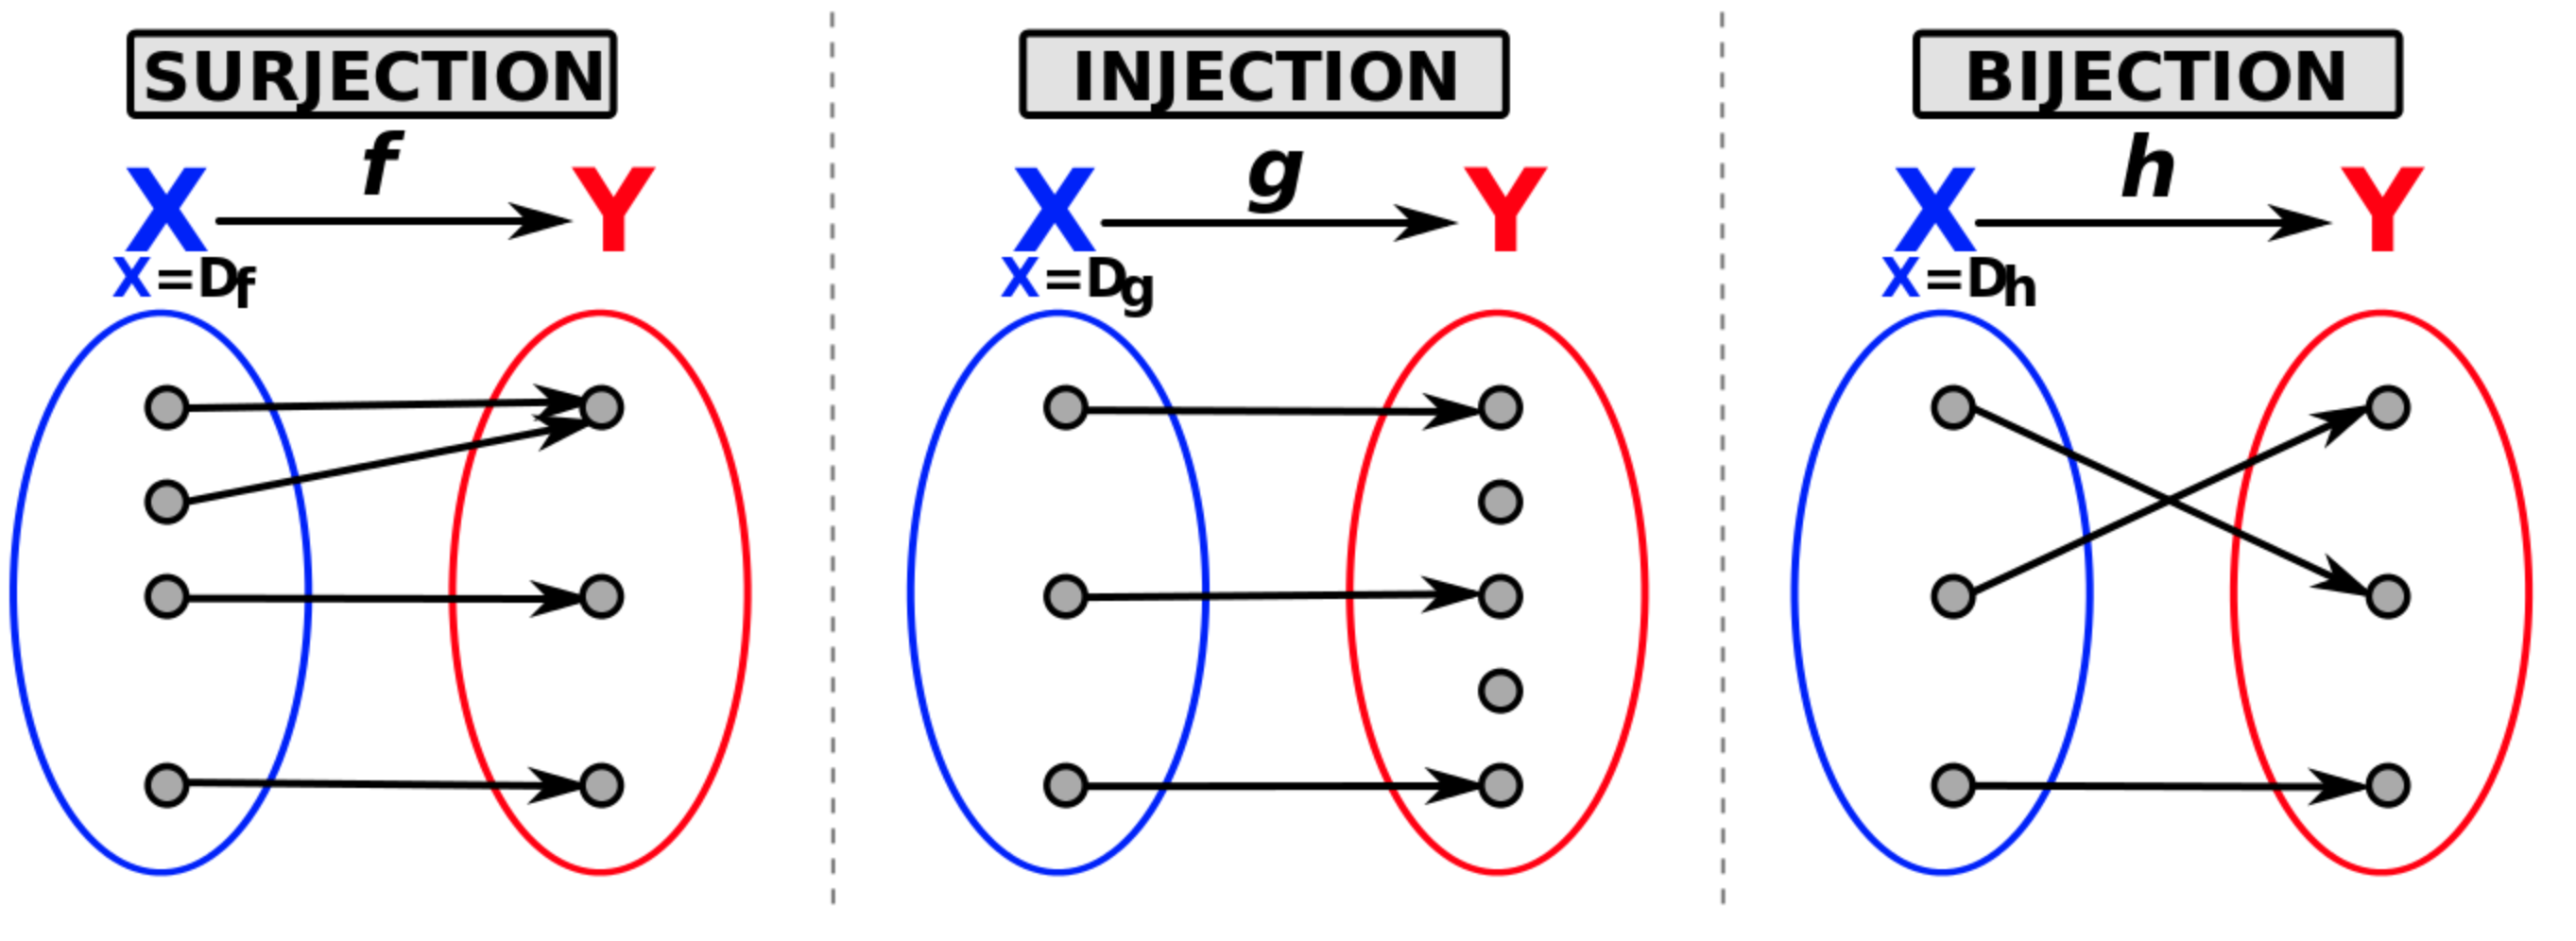
\includegraphics[scale=0.25]{figures/inj_surj_bij.png}
\end{figure}

\defn{Fonction paire}{
    $f$ est paire ssi

$$
\forall x \in D_f,\left\{\begin{array}{c}
-x \in D_f \\
f(-x)=f(x)
\end{array}\right.
$$
}


\defn{Fonction Impaire}{
    $f$ est impaire ssi

$$
\forall x \in D_f,\left\{\begin{array}{c}
-x \in D_f \\
f(-x)=-f(x)
\end{array}\right.
$$
}


\defn{Fonction périodique}{
    $f$ est périodique de période $k$ ssi

$$
\forall x \in D_f,\left\{\begin{array}{c}
x+k \in D_f \\
f(x+k)=f(x)
\end{array}\right.
$$
}

\section{Régularité}

\subsection{Continuité, Dérivabilité}
\defn{Continuité en un point}{
    $f$ est continue en un point $a \in D_f$ ssi

$$
\lim _{x \rightarrow a} f(x)=f(a) .
$$
Ou, de manière équivalente,
$$
\forall V \in \mathcal{V}(f(a)),\{x \in E \mid f(x) \in V\} \in \mathcal{V}(a)
$$
}
Ici, $V$ désigne un voisinage de $f(a)$, c'est à dire l'emsemble des réels proches de $f(a)$. Plus précisémment, 
$V \subseteq \mathbb{R}$ est un voisinage de $x_0 \in \mathbb{R}$ ssi

$$
\exists \varepsilon>0,] x_0-\varepsilon, x_0+\varepsilon[\subset V .
$$


On note $\mathcal{V}\left(x_0\right)$ l'ensemble des voisinages de $x_0$.

Une fonction est continue sur un intervalle si elle est continue en tout point de cet intervalle. 

\defn{Dérivabilité en un point}{
    $f$ est dérivable en $x \in D_f$ ssi

$$
\lim _{h \rightarrow 0} \frac{f(x+h)-f(x)}{h}
$$

existe et est finie. Cette limite est appelée dérivée de $f$ en $x$.
}

Si $f$ est dérivable en tout point d'un ensemble $H$, on dit que $f$ est dérivable sur cet ensemble $H$ et on peut définir la fonction dérivée de $f$ qui a tout point de $H$ associe la dérivée de $f$ en ce point. La fonction dérivée de $f$ est notée $f^{\prime}$ ou encore $\frac{\mathrm{d} f}{\mathrm{~d} x}$.\\

ATTENTION: "Continue", "dérivable" sont des adjectifs valabes sur un intervalle qu'il FAUT préciser !!

\subsection{Classes de régularité}

Soient $I$ un intervalle de $\mathbb{R}$ et $k$ un entier > 0.
\begin{itemize}
    \item La classe $\mathcal{C}^0(I)$ est l'ensemble des fonctions continues sur $I$.
    \item La classe $\mathcal{C}^k(I)$ est l'ensemble des fonctions $k$ fois dérivables sur $I$ et dont la $k$-ième dérivée est continue.
    \item La classe $\mathcal{C}^{\infty}(I)$ est l'ensemble des fonctions infiniment dérivables sur $I$. Ces fonctions sont aussi appelées lisses ou régulières.
\end{itemize}

En géophysique, les fonctions étudiées sont souvent supposées être "suffisament lisses" pour pouvoir les dériver autant que nécessaire.

\subsection{Propriétés et dérivées usuelles}
Soit $f$ une fonction dérivable sur un intervalle $I \subseteq \mathbb{R}$.
$f$ est croissante (au sens large) sur $I$ ssi

$$
\forall x_0 \in I, \frac{\mathrm{~d} f}{\mathrm{~d} x}\left(x_0\right) \geqslant 0
$$


De plus, $f$ est strictement croissante ssi l'ensemble des points de $I$ pour lesquels sa dérivée est nulle ne contient aucun intervalle non-trivial (un intervalle non-trivial étant un intervalle non vide et non réduit à un point). Formellement, on dit que l'intérieur de cet ensemble est nul :

$$
\operatorname{int}\left(\left\{x_0 \in I \left\lvert\, \frac{\mathrm{d} f}{\mathrm{~d} x}\left(x_0\right)=0\right.\right\}\right)=\varnothing
$$

Soit $x_0$ un point de $I$ tel que $\frac{\mathrm{d} f}{\mathrm{~d} x}\left(x_0\right)=0$. $f$ admet un minimum local en $x_0$ ssi:

$$
\exists V \in \mathcal{V}\left(x_0\right), \forall x \in V \cap I,\left\{\begin{array}{l}
x<x_0 \Longleftrightarrow \frac{\mathrm{~d} f}{\mathrm{~d} x}(x)<0 \\
x>x_0 \Longleftrightarrow \frac{\mathrm{~d} f}{\mathrm{~d} x}(x)>0
\end{array}\right.
$$

$f$ admet un maximum local en $x_0$ ssi :

$$
\exists V \in \mathcal{V}\left(x_0\right), \forall x \in V \cap I,\left\{\begin{array}{l}
x<x_0 \Longleftrightarrow \frac{\mathrm{~d} f}{\mathrm{~d} x}(x)>0 \\
x>x_0 \Longleftrightarrow \frac{\mathrm{~d} f}{\mathrm{~d} x}(x)<0
\end{array}\right.
$$

Soit $f$ et $g$ deux fonctions dérivables. On a :

$$
\begin{aligned}
\frac{\mathrm{d}}{\mathrm{~d} x}(f+g) & =\frac{\mathrm{d} f}{\mathrm{~d} x}+\frac{\mathrm{d} g}{\mathrm{~d} x} \\
\frac{\mathrm{~d}}{\mathrm{~d} x}(f g) & =f \frac{\mathrm{~d} g}{\mathrm{~d} x}+g \frac{\mathrm{~d} f}{\mathrm{~d} x} \\
\frac{\mathrm{~d}}{\mathrm{~d} x}\left(\frac{f}{g}\right) & =\frac{1}{g^2}\left(g \frac{\mathrm{~d} f}{\mathrm{~d} x}-f \frac{\mathrm{~d} g}{\mathrm{~d} x}\right) \quad(g \neq 0) \\
\frac{\mathrm{d}}{\mathrm{~d} x}(g \circ f) & =\frac{\mathrm{d}(g \circ f)}{\mathrm{d} f} \frac{\mathrm{~d} f}{\mathrm{~d} x}=\frac{\mathrm{d} g}{\mathrm{~d} x} \circ f \times \frac{\mathrm{d} f}{\mathrm{~d} x}
\end{aligned}
$$

\begin{figure}[H]
    \centering
    \begin{tabular}{|l|l|l|l|}
        \hline $f(x)$ & $D_f$ & $f^{\prime}(x)$ & $D_{f^{\prime}}$ \\
        \hline $x^n, n \in \mathbb{N}$ & $\mathbb{R}$ & $n x^{n-1}$ & $\mathbb{R}$ \\
        \hline $\frac{1}{x^n}=x^{-n}, n \in \mathbb{N}^{+}$ & $\mathbb{R}^*$ & $-\frac{n}{x^{n+1}}=-n x^{-n-1}$ & $\mathbb{R}^*$ \\
        \hline $x^\alpha, \alpha \in \mathbb{R}^{+*}$ & $\mathbb{R}^{+}$ & $\alpha x^{\alpha-1}$ & $\mathbb{R}^{+*}$ \\
        \hline $e^x$ & $\mathbb{R}$ & $e^x$ & $\mathbb{R}$ \\
        \hline $\ln |x|$ & $\mathbb{R}^*$ & $\frac{1}{x}$ & $\mathbb{R}^*$ \\
        \hline $\cos x$ & $\mathbb{R}$ & $-\sin x$ & $\mathbb{R}$ \\
        \hline $\sin x$ & $\mathbb{R}$ & $\cos x$ & $\mathbb{R}$ \\
        \hline $\tan x$ & $\mathbb{R} \backslash\left\{\frac{\pi}{2}+\pi \mathbb{Z}\right\}$ & $1+\tan ^2(x)=\frac{1}{\cos ^2(x)}$ & $\mathbb{R} \backslash\left\{\frac{\pi}{2}+\pi \mathbb{Z}\right\}$ \\
        \hline $\arccos x$ & [-1, 1] & $-\frac{1}{\sqrt{1-x^2}}$ & ] - 1, 1[ \\
        \hline $\arcsin x$ & [-1, 1] & $\frac{1}{\sqrt{1-x^2}}$ & ] - 1, 1[ \\
        \hline $\arctan x$ & $\mathbb{R}$ & $\overline{1+x^2}$ & $\mathbb{R}$ \\
        \hline $\cosh x$ & $\mathbb{R}$ & $\sinh x$ & $\mathbb{R}$ \\
        \hline $\sinh x$ & $\mathbb{R}$ & $\cosh x$ & $\mathbb{R}$ \\
        \hline $\tanh x$ & $\mathbb{R}$ & $1-\tanh ^2(x)=\frac{1}{\cosh ^2(x)}$ & $\mathbb{R}$ \\
        \hline
        \end{tabular}
\end{figure}


\section{Développements limités}
\subsection{Les notations de Landau}
Ce sont des notations communément utilisées pour comparer asymptotiquement des expressions. Considérons deux fonctions $f$ et $g$.Vons devez connaître:

\begin{itemize}
    \item $f(x) = O(g(x))$ : "f est un grand O de g": il existe un certain rang de $x$ à partir duquel $|f(x)| < |g(x)|$.
    $$\exists k>0, \exists x_0 \forall x>x_0|f(x)| \leq|g(x)| \cdot k$$
    \item $f(x) = o(g(x))$ : "f est un petit o de g": f est négligeable devant g
    $$\forall \varepsilon>0 \exists x_0 \forall x>x_0|f(x)| \leq|g(x)| \cdot \varepsilon$$
    \item $f(x) \sim g(x)$: "f est équivalente à g"
    $$\forall \varepsilon>0 \exists x_0 \forall x>x_0|f(x)-g(x)|<\varepsilon|g(x)|$$
\end{itemize}

\subsection{Définition d'un développement limité}
On dit qu'une fonction $f$ admet un développement limité d'ordre $n$ (abbrégé $D L_n$ ) au voisinage de $x_0$ ssi :

$$
\exists\left(\begin{array}{c}
a_0 \\
\vdots \\
a_n
\end{array}\right) \in \mathbb{R}^{n+1}, \exists V \in \mathcal{V}\left(x_0\right), \forall x \in V, \quad f(x)=\sum_{k=0}^n a_k\left(x-x_0\right)^k+o\left(\left(x-x_0\right)^n\right)
$$


Le $D L_n$ d'une fonction est composé d'un polynôme d'ordre $n$ et d'un reste $o\left(\left(x-x_0\right)^n\right)$ tel que (notation "petit o" de Landau) :

$$
\lim _{x \rightarrow x_0} \frac{o\left(\left(x-x_0\right)^n\right)}{\left(x-x_0\right)^n}=0 .
$$

\defn{Série de Taylor}{
    Soit $f \in \mathcal{C}^{\infty}$ et $x_0 \in D_f$. La série de Taylor de $f$ en $x_0$ est la série entière

$$
T_{x_0}^f(x)=\sum_{n=0}^{\infty} \frac{f^{(n)}\left(x_0\right)}{n!}\left(x-x_0\right)^n
$$

où $f^{(n)}=\frac{\mathrm{d}^n f}{\mathrm{~d} x^n}$ est la $n$-ième dérivée de $f$.
}


$f$ est analytique en $x_0$ ssi

$$
\exists V \in \mathcal{V}\left(x_0\right), \forall x \in V, f(x)=T_{x_0}^f(x)
$$

$f$ est entière ssi

$$
\forall x_0 \in \mathbb{R}, \forall x \in \mathbb{R}, f(x)=T_{x_0}^f(x) .
$$

Soient un intervalle $I \subseteq \mathbb{R}$ et $f$ une fonction de classe $\mathcal{C}^n(I)$.

$$
\forall x_0 \in I, \exists V \in \mathcal{V}\left(x_0\right), \forall x \in V \cap I, \quad f(x)=\sum_{k=0}^n \frac{f^{(k)}\left(x_0\right)}{k!}\left(x-x_0\right)^k+o\left(\left(x-x_0\right)^n\right)
$$


En géophysique, les fonctions étudiées sont souvent supposées être de classe $\mathcal{C}^n$. On se sert alors des premiers termes de la série de Taylor pour approximer ces fonctions sous une forme polynômiale. En particulier, l'approximation linéraire utilisant un DL d'ordre 1 peut s'écrire :

$$
f\left(x_0+h\right) \approx f\left(x_0\right)+h \frac{\mathrm{~d} f}{\mathrm{~d} x}\left(x_0\right)
$$

\subsection{DL usuels}

\begin{align} 
    e^x & =1+\frac{x}{1!}+\frac{x^2}{2!}+\cdots+\frac{x^n}{n!}+o\left(x^n\right) \\ 
    \operatorname{ch} x & =1+\frac{x^2}{2!}+\frac{x^4}{4!}+\cdots+\frac{x^{2 n}}{(2 n)!}+o\left(x^{2 n+1}\right) 
    \\ \operatorname{sh} x & =x+\frac{x^3}{3!}+\frac{x^5}{5!}+\cdots+\frac{x^{2 n+1}}{(2 n+1)!}+o\left(x^{2 n+2}\right) \\
    \operatorname{th} x & =x-\frac{x^3}{3}+\frac{2}{15} x^5-\frac{17}{315} x^7+o\left(x^8\right) \\
    \cos x & =1-\frac{x^2}{2!}+\frac{x^4}{4!}+\cdots+(-1)^n \cdot \frac{x^{2 n}}{(2 n)!}+o\left(x^{2 n+1}\right) \\
    \sin x & =x-\frac{x^3}{3!}+\frac{x^5}{5!}+\cdots+(-1)^n \cdot \frac{x^{2 n+1}}{(2 n+1)!}+o\left(x^{2 n+2}\right) \\
    \tan x & =x+\frac{x^3}{3}+\frac{2}{15} x^5+\frac{17}{315} x^7+o\left(x^8\right) \\
    (1+x)^\alpha & =1+\alpha x+\frac{\alpha(\alpha-1)}{2!} x^2+\cdots+\frac{\alpha(\alpha-1) \cdots(\alpha-n+1)}{n!} x^n+o\left(x^n\right)\\
    \frac{1}{1+x} & =1-x+x^2+\cdots+(-1)^n x^n+o\left(x^n\right) \\
    \sqrt{1+x} & =1+\frac{x}{2}-\frac{1}{8} x^2+\cdots+(-1)^{n-1} \cdot \frac{1.1 .3 .5 \cdots(2 n-3)}{2^n n!} x^n+o\left(x^n\right) \\
    \frac{1}{\sqrt{1+x}} & =1-\frac{x}{2}+\frac{3}{8} x^2+\cdots+(-1)^n \cdot \frac{1.3 .5 \cdots(2 n-1)}{2^n n!} x^n+o\left(x^n\right) \\
    \ln (1+x) & =x-\frac{x^2}{2}+\frac{x^3}{3}+\cdots+(-1)^{n-1} \cdot \frac{x^n}{n}+o\left(x^n\right) \\
    \operatorname{argth} x & =x+\frac{x^3}{3}+\frac{x^5}{5}+\cdots+\frac{x^{2 n+1}}{2 n+1}+o\left(x^{2 n+2}\right) \\
    \arctan x & =x-\frac{x^3}{3}+\frac{x^5}{5}+\cdots+(-1)^n \cdot \frac{x^{2 n+1}}{2 n+1}+o\left(x^{2 n+2}\right) \\
    \operatorname{argsh} x & =x-\frac{1}{2} \frac{x^3}{3}+\frac{3}{8} \frac{x^5}{5}+\cdots+(-1)^n \cdot \frac{1.3 .5 \cdots(2 n-1)}{2^n n!} \frac{x^{2 n+1}}{2 n+1}+o\left(x^{2 n+2}\right) \\
    \arcsin x & =x+\frac{1}{2} \frac{x^3}{3}+\frac{3}{8} \frac{x^5}{5}+\cdots+\frac{1.3 .5 \cdots(2 n-1)}{2^{2 n+1}}+o\left(x^{2 n+2}\right)
\end{align}